\begin{figure*}[t]
\centering
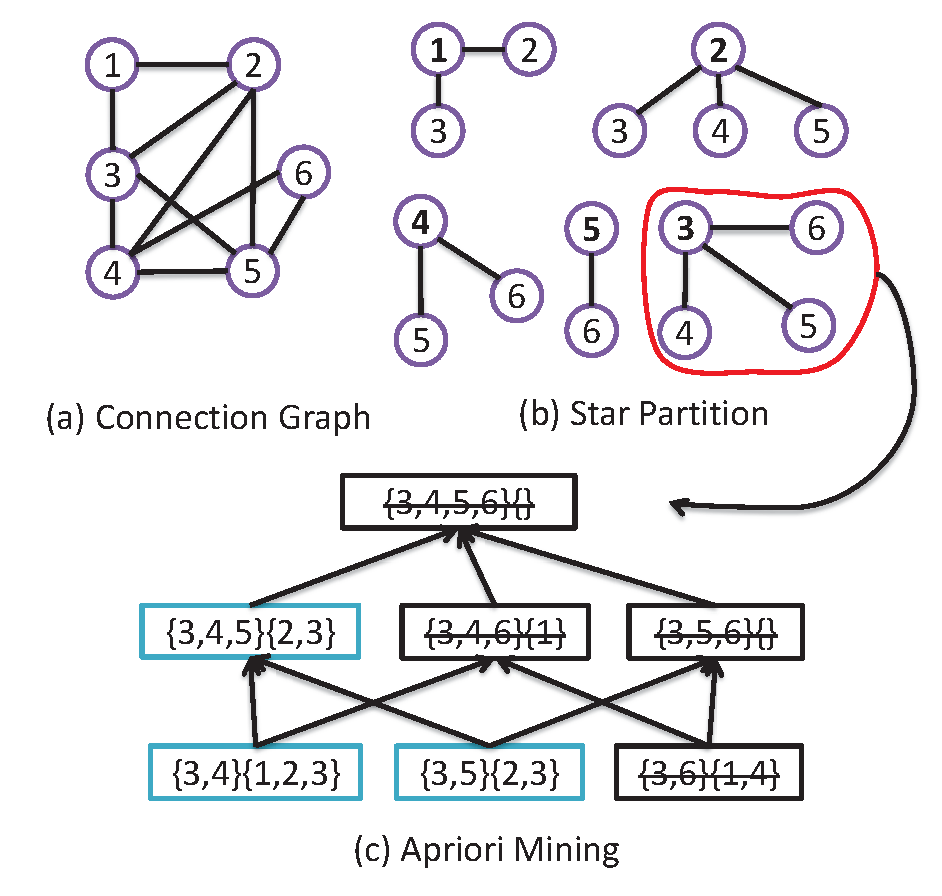
\includegraphics[width=0.9\textwidth]{spm.eps}
\caption{Star partition and mining. (a) Conceptual connection graph from Figure 1.(b) Five star partitions are generated
(c) Apriori Mining with various pruning techniques.}
\label{fig:star_partition}
\end{figure*}

\section{SPARE: Star Partitioning and Apriori Enumerator}
\label{sec:spm}
The aforementioned replicate partitioning is based on the temporal dimension which suffers from two drawbacks. First, the replication relies on $\eta$ which could be large. Second, the same valid pattern may be discovered from different partitions which results in redundant work.
%and results in groups of snapshots in each partition.
% ADD MORE DETAILS ABOUT THE LIMITATIONS HERE.
To resolve the limitations caused by the replicate partitioning, 
we propose a new Star Partitioning and ApRiori Enumerator, named SPARE, 
to replace the second cycle of map-reduce jobs in Figure~\ref{fig:trm}. 
Our new parallel mining framework is shown in Figure~\ref{fig:star_partition}. 
Its input is the set of clusters generated in each snapshot and the output 
contains all the valid GCMP patterns. In the following, we explain the two major components: 
star partitioning and apriori enumerator.


\subsection{Star Partitioning}
Let $G_t$ be a graph for snapshot $S_t$, in which each node 
is a moving object and two objects are connected if they appear 
in the same cluster. It is obvious that $G_t$ consists of a set of small cliques. 
Based on $G_t$, we define an aggregated graph $G_A$ to summarize the 
cluster relationship among all the snapshots. In $G_A$, two objects
form an edge if they are connected in any $G_t$s. Furthermore, 
we attach an inverted list for each edge, 
storing the associated timestamps in which the two objects are connected. 
An example of $G_A$, built on the trajectory database in Figure~\ref{fig:related_work}, 
is shown in Figure~\ref{fig:star_partition} (a). 
As long as two objects are clustered in any timestamp, they are connected in $G_A$. 
The object pair $(o_1,o_2)$ appears in two clusters at timestamps 
$2$ and $3$ and is thus associated with an inverted list $\{2,3\}$.


We use \emph{star} as the data structure to capture the pair relationships. 
To avoid duplication, as $G_t$ is an undirected graph and an edge may appear in multiple stars, 
we enforce a global ordering among the objects and propose a concept named \textit{directed star}.

\begin{definition}[Directed Star]
Given a vertex with global id $s$, its directed star $Sr_s$ is defined as the set of neighboring vertices with global id $t>s$. We call $s$ the star ID.
\end{definition}

With the global ordering, we can guarantee that each edge is contained in a unique star partition. Given the aggregated graph $G_A$  in Figure~\ref{fig:star_partition} (a), we enumerate all the possible directed stars in Figure~\ref{fig:star_partition} (b). These stars are emitted from mappers to different reducers. The key is the star ID and the value is the neighbors in the star as well as the associated inverted lists. 
The reducer will then call the Apriori-based algorithm to enumerate all the valid GCMP patterns.


Before we introduce the Apriori enumerator, we are interested to 
examine the issue of global ordering on the moving objects.
This is because assigning different IDs to the objects will result in 
different star partitioning results, which will eventually affect the workload 
balance among the map-reduce jobs. The job incurring performance bottleneck is often known as \emph{straggler}~\cite{kwon2012skewtune,xin2013shark,coppa2015data}. In the context of star partitioning, a straggler refers to the job assigned with the maximum star partition. We use $\Gamma$ to denote the size of a partition and $\Gamma$ is set to the number of edges in a directed star\footnote{A star is essentially a tree structure and the number of nodes equals the number of edges minus one.}. It is straightforward that a star partitioning with small $\Gamma$ is preferred. For example, Figure~\ref{fig:star-alt} gives two star partitioning results under 
different vertex ordering on the same graph. The top one has $\Gamma = 5$ while the bottom one has $\Gamma = 3$. Obviously, the bottom one with smaller $\Gamma$ is much more balanced.


%An important concern in design parallel algorithms is the distribution of work loads.  
%Traditionally, the quality of a partition strategy 
%is measured based on two aspects: (1) the number of result partition, which
%affects the maximum parallelism
%(2) the size balance of partitions, which affects the finishing
%time of a job. Unlike TRM where each partition
%contains equal-sized snapshots, the size distribution 
%of stars in SPM remains unknown.
%Nevertheless, we notice that, in SPM, the total sizes of 
%stars are invariant. Therefore, the quality of a star partition
%can be formalized as the \emph{skewness}, which is the maximum star size
%among all stars. Smaller \emph{skewness} naturally results in more partitions
%and less imbalance.
%}

\begin{figure}[h]
\centering
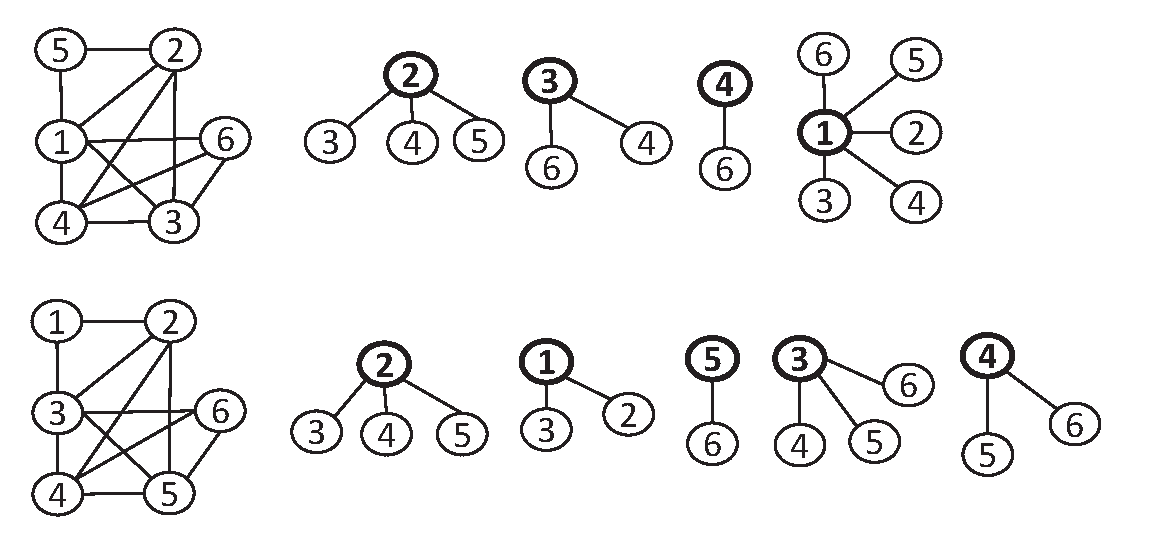
\includegraphics[width=0.5\textwidth]{star-alt.eps}
\caption{Examples of star partitioning with different vertex ordering.}
\label{fig:star-alt}
\end{figure}


%To determine the optimal vertex orders with the objective of minimizing $\Gamma$, 
%we can use a linear algebra model as follows:  
%Let $G_A$ be an aggregate graph, with a $n \times n$ adjacent matrix $J$.
%A vertex order is in fact a permutation of $J$. Therefore,
%the adjacent matrices of any reordered graphs can be represented as $PJP^T$
%where $P \in \mathbb{P}$ is a 
%\emph{permutation matrix}~\footnote{an identity matrix with rows shuffled} with dimension $n$.
%Since in star partition, we assign each edge $e(i,j)$ in $G_A$ to the lower vertex, 
%then the matrix $B=\triu(PJP^T)$~\footnote{\text{triu} is the upper triangle part of a matrix}
%represents the assignment matrix wrt. $P$ (i.e., $b_{i,j} = 1$ if vertex $j$ is in star $Sr_i$).
%Let vector $\vec{b}$ be the \textit{one}\footnote{every element in $\vec{b}$ is $1$} 
%vector of size $n$. Let $\vec{c} = B\vec{b}$, then each $c_i$ 
%denotes the number of edges in star $Sr_i$. Thus, $\Gamma$ can be represented
%as the infinity norm of $B\vec{b}$. Let $\Gamma^*$ be the minimum $\Gamma$ among all vertex orders. 
%$\Gamma^*$ can then be formulated as follows:
%\begin{equation}
%\Gamma^* = \min_{P \in \mathbb{P}}{||B\vec{b}||_\infty} \text{ ,where } ||B\vec{b}||_\infty = \max_{1\leq j \leq n}(c_j)
%\end{equation}

Although it is very challenging to find the optimal vertex id ordering from the $n!$ possibilities, we observe that a random order can actually achieve satisfactory performance based on the following theorem.



\begin{theorem}
\label{THM:SPM_LB}
Let $\Gamma^*$ be the value derived from the optimal vertex ordering and  $\Gamma$ be value derived from a random vertex ordering. With probability $1-1/n$, we have $\Gamma = \Gamma^* + O(\sqrt{n \log n})$.
\end{theorem}
\begin{proof}
In Appendix XXX.
\end{proof}
If $G_A$ is a dense graph, we can get a tighter bound for $(\Gamma - \Gamma^*)$.
\begin{theorem}
\label{THM:SPM_LB_INC}
Let $d$ be the average degree in $G_A$. If $d\geq \sqrt{12\log n}$, with
high probability $1-1/n$, $\Gamma = \Gamma^* + O(\sqrt{d\log n})$.
\end{theorem}
\begin{proof}
In Appendix XXXX.
\end{proof}
Hence, we can simply use object id to determine the vertex ordering in our implementation.


%
%Even though the TRM algorithm works in a parallel way, it requires to replicate the data $\eta$ times. 
%When $\eta$ is small, TRM perform good parallelism. However, wh
%
%When handling \emph{swarm}, \emph{group} and \emph{platoon} patterns, $\eta$ has to be set to $|\mathbb{T}|$ to guarantee correctness, resulting in very expensive data replication overhead. 
%%Handling those cases are equivalent to replicate the entire snapshots to each partition, 
%%which surrenders the benefit of parallelism.
\eat{
Although TRPM works in a parallel way, we observe two inefficiencies. First, the
performance of TRPM largely relies on $\eta$ which further depends on pattern parameters.
When $\eta$ is large, the shuffle and reduce cost of TRPM is high. Second, 
the parallel execution of line sweep algorithm may discover the same pattern from
multiple partitions, which introduces redundant work. To resolve the two limitations,
we design a novel \emph{Star Partition and Mining} algorithm.
}
%After computing the star, each partition is applied with a reduce task. 
%Indeed, a star $Sr_s$ can be viewed as a subset of original trajectories. 
%This is done by treating each vertex in $Sr_s$ as an object. 
%The time sequence of $s$ is the union of all edges in $Sr_s$. 
%And the time sequence of $v \neq s$ is the edge $(s,v)$. Therefore, we
%are able to mine stars from the similar trajectory concepts.

\subsection{Apriori Enumerator}
Intuitively, given a GCMP pattern with an object set $\{o_1,o_2,\ldots,o_m\}$, 
all the pairs of $(o_i,o_j)$ with $1\leq i<j\leq m$ must 
be connected in the associated temporal graphs $\{G_t\}$. This inspires us to leverage the classic Apriori algorithm to enumerate all the valid GCMP patterns starting from pairs of objects. However, we observe that the monotonicity property does not hold between an object set and its supersets.

\begin{example}
In this example, we show that if an object set is not a valid pattern, we cannot prune all its super sets.
Consider two candidates $P_1=\{o_1,o_2:1,2,3,6\}$ and $P_2=\{o_1,o_3:1,2,3,7\}$. 
Let $L=2,K=3$ and $G=2$. Both candidates are not valid patterns because the constraint on $L$ is not satisfied. 
However, when considering their object superset $\{o_1,o_2,o_3\}$, we can infer that their co-clustering timestamps are in $(1,2,3)$. This is a valid pattern conforming to the constraints of $L,K,G$. Thus, we need a new type of monotonicity to facilitate pruning.
\end{example}   


\subsubsection{Monotonicity}
To ensure the monotonicity, we first introduce a procedure named \textit{star simplification}, to reduce the number of edges as well as unnecessary timestamps in the inverted lists. For instance, if the size of the inverted list for an edge $e$ is smaller than $K$, then the edge can be safely removed because the number of timestamps in which its supersets are clustered must also be smaller than $K$. To generalize the idea, we propose three concepts named \textit{maximal $G$-connected subsequence}, \emph{decomposable sequence} and \emph{sequence simplification}.

\begin{definition}[Maximal $G$-connected Subsequence]
A sequence $T'$ is said to be a maximal $G$-connected subsequence of $T$ if (1) $T'$ is the subsequence of $T$, i.e., $\exists i\leq j, T' = T(i,\ldots,j)$ , (2) $T'$ is $G$-connected, and (3) there exists no other subsequence $T''$ of $T$ such that $T'$ is the subsequence of $T''$ and $T''$ is G-connected.
\end{definition}
%Hence, our idea is to examine the validity of object pairs. If $(o_i,o_j)$ itself is not a valid GCMP pattern, then all the supersets containing $(o_i,o_j)$ can be pruned. For instance, $(XXX,XXX)$ are not connected in Figure~\ref{} and all its supersets can be pruned.

\begin{example}
Suppose $G=2$ and consider two sequences $T_1=(1,2,4,5,6,9,10,11,13)$ and $T_2=(1,2,4,5,6,8,9)$. $T_1$ has two maximal $2$-connected subsequences:$T_1^A=(1,2,4,5,6)$ and $T_1^B=(9,10,11,13)$. This is because the gap between $T_1^A$ and $T_1^B$ is $3$ and it is impossible for the timestamps from  $T_1^A$ and $T_1^B$ to form a new subsequence with $G\leq 2$. Since $T_2$ is $2$-connected, $T_2$ has only one maximal $2$-connected subsequence which is
itself. 
\end{example}

The maximal $G$-connected subsequence has the following two properties:
\begin{lemma}\label{lemma:union-property}
Suppose $\{T_1,T_2,\ldots,T_m\}$ is the set of all maximal $G$-connected subsequences of $T$, we have (1) $T_i\cap T_j=\emptyset$ for $i\neq j$ and (2) $T_1\cup T_2\cup\ldots\cup T_m=T$.
\end{lemma}
\begin{proof}
We assume $T_i\cap T_j\neq \emptyset$. Let $T_i=(T_i[1], T_i[2],\ldots,T_i[p])$ and $T_j= (T_j[1], T_j[2],\ldots,T_j[n])$. Suppose $T[x]$ is a timestamp occurring in both $T_i$ and $T_j$. Let $T[y]=\min\{T_i[1],T_j[1]\}$, i.e., the minimum timestamp of $T_i[1]$ and $T_j[1]$ occurs at the $y$-th position of sequence $T$. Similarly, we assume $T[z]=\max\{T_i[p], T_j[n]\}$. Apparently, the two subsequences $T[y:x]$ and $T[x:z]$ are $G$-connected because $T_i$ and $T_j$ are both $G$-connected. Then, sequence $(T_y,\ldots,T_x,\ldots,T_z)$, the superset of $T_i$ and $T_j$, is also $G$-connected. This contradicts with the assumptions that $T_i$ and $T_j$ are maximal $G$-connected subsequences. 




To prove (2), we assume $\cup_i T_i$ does not cover all the timestamps in $T$. Then, we can find a subsequence $T'=T[x:x+t]$ such that $T[x-1]\in T_a$ $(1\leq a\leq m)$, $T[x+t+1]\in T_b$ $(1\leq b\leq m)$ and all the timestamps in $T'$ is not included in any $T_i$. Let $g'=\min\{T[x]-T[x-1], T[x+t+1]-T[x+t]\}$. If $g'\leq G$, then it is easy to infer that $T_a$ or $T_b$ is not a maximal $G$-connected subsequence because we can combine it with $T[x]$ or $T[x+t]$  to a form superset which is also $G$-connected. If $g'>G$, $T'$ itself is a maximal $G$-connected subsequence which is missed in $\cup T_i$. Both cases lead to contradiction.
\end{proof}




\begin{lemma}\label{lemma:subset-property}
If $T_1$ is a subset of $T_2$, then for any maximal $G$-connected subsequence $T_1'$ of $T_1$, we can find a maximal $G$-connected subsequence $T_2'$ of $T_2$ such that $T_1'$ is a subset of $T_2'$.
\end{lemma}
\begin{proof}
Since $T_1' \subseteq T_1 \subseteq T_2 $, we know $T_1'$ is a $G$-connected subsequence of $T_2$. Based on Lemma~\ref{lemma:union-property}, we can find a maximal $G$-connected subsequence of $T_2$, denoted by $T_2'$, such that $T_1'\cap T_2'\neq \emptyset$. If there exists a timestamp $T_1'[x]$ such that $T_1'[x]\notin T_2'$, similar to the proof of case (1) in Lemma~\ref{lemma:union-property}, we can obtain a contradiction. Thus, all the timestamps in $T_1'$ must occur in $T_2'$.
\end{proof}

\begin{definition}[Decomposable Sequence]
$T$ is decomposable if for any of its maximal $G$-connected subsequence $T'$, we have (1) $T'$ is $L$-consecutive; and (2) $|T'|\geq K$.
\end{definition}

\begin{example}
Let $L = 2, K = 4$ and we follow the above example. $T_1$ is not a decomposable sequence
because one of its maximal $2$-connected subsequence (i.e., $T_1^B$) is not $2$-consecutive.
In contrast, $T_2$ is a decomposable sequence because the sequence itself is the maximal $2$-connected subsequence, which is also $2$-consecutive and with size no smaller than than $4$.
\end{example}


%Not that, although $T_1$ is not a candidate sequence, it can be simplified
%to a candidate sequence (i.e, $T_2$). Generally, for any time sequence $T$, 
%if it does not contain a \emph{candidate sequence}, then it cannot contribute
%to any valid patterns. In fact, only the candidate sequence inside $T$ affects
%the final patterns. Therefore, we may use the candidate sequence to simplify edges in 
%a star. During the simplification, if an edge results in a candidate
%sequence of size zero, then it is removed from the star. Otherwise,
%the simplified edge is kept. By so doing, the size of the new star
%is much smaller.

\begin{definition}[Sequence Simplification]
Given a sequence $T$, the simplification procedure $\mathtt{sim}(T) =  g_{G,K} \cdot f_L(T) $ can be seen as a composite function with two steps: 
\begin{enumerate}
\item $f$-step: remove segments of $T$ that are not $L$-consecutive;
\item $g$-step: among the maximal $G$-connected subsequences of $f_L(T)$, remove those with size smaller than $K$.
\end{enumerate}
\end{definition}


\begin{example}
Take $T=(1,2,4,5,6,9,10,11,13)$ as an example for sequence simplification. 
Let $L = 2, K = 4$ and $G = 2$. In the $f$-step, $T$ is reduced to $f_2(T)=(1,2,4,5,6,9,10,11)$. 
The segment $(13)$ is removed due to the constraint of $L=2$. 
$f_2(T)$ has two maximal $2$-consecutive subsequences: $(1,2,4,5,6)$ and $(9,10,11)$. 
Since $K=4$, we will remove $(9,10,11)$ in the $g$-step. Finally, the output is $\mathtt{sim}(T)=(1,2,4,5,6)$.
\end{example}

It is possible that the simplified sequence $\mathtt{sim}(T)=\emptyset$. For example, Let $T=(1,2,5,6)$ 
and $L=3$. All the segments will be removed in the $f$-step and the output is $\emptyset$.
We define $\emptyset$ to be not decomposable. 
%Based on the above definitions, we can define our monotonicity to facilitate the pruning in the Apriori algorithm.
We provide an important property of the sequence simplification process as follows:
\begin{lemma}\label{lemma:decom-sim}
If sequence $T$ is a superset of any decomposable sequence, then $\mathtt{sim}(T) \neq \emptyset$.
\end{lemma}
\begin{proof}
It is obvious that $\mathtt{sim}(T)$ is a one-to-one function. Given an input sequence T, there is a unique  $\mathtt{sim}(T)$. Let $T_p$ be a decomposable subset of $T$ and we prove the lemma by showing that $\mathtt{sim}(T)$ is a superset of $T_p$.

Suppose $T_p$ can be decomposed into a set of maximal $G$-connected
subsequences $T_p^1, \ldots, T_p^m$ ($m \geq 1$). Since $T_p$ is a subset of $T$, all the $T_p^i$ are also subsets of $T$. By definition, each $T_p^i$ is $L$-consecutive. Thus, in the $f$-step of $\mathtt{sim}(T)$, none of $T_p^i$ will be removed. In the $g$-step, based on Lemma~\ref{lemma:subset-property}, we know that each $T_p^i$ has a superset in the maximal $G$-connected subsequences of $f_L(T)$. Since $|T_p^i|\geq K$, none of $T_p^i$ will be removed in the $g$-step. Therefore, all the $T_p^i$ will be retained after the simplification process and $\mathtt{sim}(T) \neq \emptyset$.
\end{proof}



\eat{
Nevertheless, if there exists a $T^\#$ of $T$, then $T^\#$ is unique
as stated in the following theorem:
\begin{theorem}
For any sequence $T$, if $T$'s simplified sequence is not empty, then
there exists a unique $T^\#$ wrt $T$.
\end{theorem}
\begin{proof}
We prove by contradiction. Suppose there are two simplified sequences $T_A^\#$ and $T_B^\#$ of the same $T$. We prove that, unless $T_B^\# \equiv T_A^\#$, $T_A^\#$ can always be enlarged, which leads to a contradiction. For simplicity, we use $\overline{ab}$ to denote the segment of a sequence from timestamp $a$ to timestamp $b$.
Consider the timestamps $T_C=T_B^\# - T_A^\#$. If $T_C = \emptyset$, then $T_A^\# \equiv T_B^\#$ naturally.

Next, since $T_C \not \equiv \emptyset$, W.L.O.G, let the first timestamp in $T_A^\#$ be greater than the first timestamp $T_B^\#$. Consider the general setting: $\overline{ab}$ is the first candidate sequence in $T_A^\#$;  $\overline{ef}$
is a consecutive sequence in $T_C$ and $f < a$; $\overline{cd}$ is the next candidate sequence of $\overline{ef}$ in $T_B^\#$; $\overline{gh}$ is the previous candidate sequence of $\overline{ef}$ in $T_B^\#$; Categorize on the gaps between $\overline{ef}$ and  $\overline{cd}$, $\overline{gh}$,
there are four cases to be considered. 
We demonstrate the cases in Figure~\ref{fig:proof_thm_3}:
\begin{figure}[h]
\centering
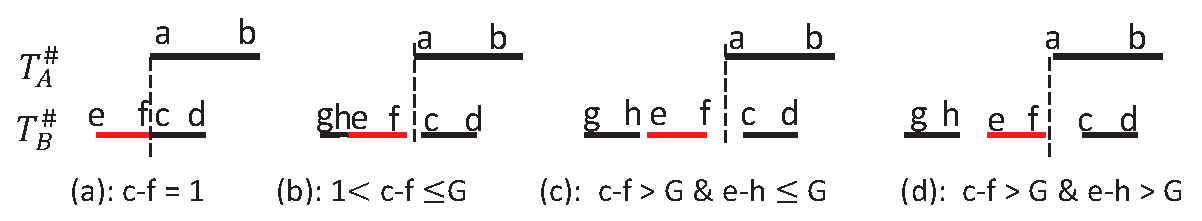
\includegraphics[width=0.46\textwidth]{thm3proof.eps}
\caption{Proof of theorem 3 with the four cases.}
\label{fig:proof_thm_3}
\end{figure}
\begin{itemize}
\item Case (a): $c-f = 1$, that is $\overline{ef}$ is part of a longer consecutive segment $\overline{ed}$. Since timestamp $c$ is in $T_A^\#$, $T_A^\#$ can be safely enlarged by increasing $\overline{ab}$ to $\overline{eb}$.
\item Case (b): $G \geq c-f> 1$. In this case, since $c\geq a$, then $a-f \leq G$. Further, since $\overline{ed}$ is not 
consecutive, $\overline{ef}$ must belongs to a larger consecutive segment $\overline{gf}$ with size no less than $L$. Therefore, adding $\overline{gf}$ to $\overline{ab}$ makes $\overline{gb}$ still a candidate sequence.
\item Case (c): $c-f > G$ and $e-h \leq G$. In this case, $\overline{ef}$ belongs to a candidate sequence $\overline{gf}$ in $T_B^\#$.  Since $\overline{gf}$ has no intersection with $\overline{ab}$, then adding $\overline{gf}$ to $T_A^\#$ is valid.
\item Case (d): $c-f > G$ and $ e- h > G$. In this case,  $\overline{ef}$ has to be a candidate sequence. Since $\overline{ef}$ has no intersection with $\overline{ab}$, adding $\overline{ef}$ to $\overline{ab}$ is valid.
\end{itemize}
In all cases, $T_A^\#$ can be enlarged, which contradicts with the assumption $T_A^\#$ is the simplified sequence. This completes the proof.
\end{proof}
}



\eat{
Next, we design an efficient simplification process with linear complexity.
It takes two rounds scan of $T$ as shown in Algorithm~\ref{algo:simp_prune}. 
In the first round, the consecutive portions of $T$ with size less than $L$ are removed.
In the second round, the maximal $G$-connected sequences of size less than $K$ are removed. 

\begin{algorithm}
\caption{Edge Simplification}
\label{algo:simp_prune}
\begin{algorithmic}[1]
\Require $T$
\State{---$L$ Phase---}
\State $c \gets 0$
\For {$i \in (0,...,|T|)$}
	\If{$T[i] - T[i-1] > 1$} 
		\If{$i - c < L$} 
			\State $T$ remove $[c:i)$
		\EndIf
		\State $c \gets i$
	\EndIf
\EndFor
\State{---$G$-$K$ Phase---}
\State $s\gets 1$, $c\gets 0$
\For{$i \in (0: |T|)$}
	\If{$T[i] - T[i-1] > G$}
		\If{$s < K$}   
			\State $T$ remove $[c:i)$
		\EndIf
		\State {$c \gets i$, $s \gets 1$}
	\Else
		\State $s++$
	\EndIf
\EndFor
\end{algorithmic}
\end{algorithm}
}

With Lemma~\ref{lemma:decom-sim}, we are ready to define the \emph{monotonicity} based on the simplified
sequences to facilitate the pruning in the Apriori algorithm. 

\begin{theorem}[Monotonicity]\label{THM:SPARE_MONO}
Given a candidate pattern $P=\{O:T\}$, if $\mathtt{sim}(P.T)=\emptyset$, then any pattern candidate $P'$ with $P.O \subseteq P'.O$ can be pruned.
\end{theorem}

\begin{proof}
We prove by contradiction. Suppose there exists a valid pattern $P_2$ such that $P_2.O \supseteq P.O$. It is obvious that $P_2.T \subseteq P.T$. Based on the Definition 2, the following conditions hold: (1) $P_2.T$ is $G$-connected. (2) $|P_2.T| \geq K$ and (3) $P_2.T$ is $L$-consecutive. Note that the entire $P_2.T$ is $G$-connected. Thus, $P_2.T$ itself is the only maximal $G$-connected subsequence. Based on conditions (1),(2),(3) and Definition 6, $P_2.T$ is decomposable. Then, based on Lemma~\ref{lemma:decom-sim}, we know $\mathtt{sim}(T)\neq \emptyset$ because $P_2.T \subseteq P.T$ and $P_2.T$ is decomposable. This leads to a contradiction with $\mathtt{sim}(P.T)=\emptyset$.
\end{proof}

%IN THE PROOF, YOU NEED TO SHOW 1) $P$ IS NOT VALID 2) ALL THE SUPERSETS OF $P.O$ ARE NOT VALID.












\subsubsection{Apriori Enumeration}
We then design the Apriori enumeration method to
systematically discover all valid patterns in a star.
%During the enumeration, we refer a candidate pattern
%$P$ as a $R$-candidate if $|P.O|=R$.
The enumeration method discover patterns iteratively using ``bottom-up'' order:
candidates with smaller objects set grow one object per iteration.
%
%in iteration $i$,  all $(i+1)$-candidates grows
%to $(i+2)$-candidates.
%
Enumeration ends if no
further candidates can be generated.

 Due the \emph{monotonicity} proved in Theorem~\ref{THM:SPARE_MONO}, we are able to use the \emph{monotonic pruning} and \emph{forward closure check} to boost the enumeration process. We show the detail of the process
in Algorithm~\ref{algo:apriori_mining}. As a start, 
each input edge is treated as a candidate pattern, with the 
inverted list as the time sequence. These candidates
are kept in $\mathbf{G}$ as the ground set (Lines~\ref{code:init-start}-\ref{code:init-end}). In initialization, the inverted lists are simplified (Line~\ref{code:simp1}) and unqualified lists are pruned (Line~\ref{code:init-prune}). Throughout the algorithm, we maintain a set of candidates $\mathbf{C}$ which is initialized to the ground set $\mathbf{G}$ (Line~\ref{code:init-C}). 

In each iteration (Lines~\ref{code:level-start}-\ref{code:level-ends}),  the members in candidate set are joined with the members in ground set to generate new candidates (Lines~\ref{code:join-start}-\ref{code:join-ends}). The join of two candidates $c$ and $g$ creates a 
new candidate, whose objects are the union of $c.O$ and$g.O$ and the time sequence is the intersection of $c.T$ and $g.T$ (Line~\ref{code:join}). During the join,
we use \emph{sequence simplification} to detect unqualified candidates. By \emph{monotonicity}, these candidates are safely excluded from the future iterations~(Line~\ref{code:mono-pruning}). If a valid candidate is not able to be extended by any ground set, we directly output it (Line~\ref{code:output1}). 

After the join finishes, we start a \emph{forward closure} check (Lines~\ref{code:fc-checking-start}-\ref{code:fc-checking-ends}). We test whether the union of all candidates in $\mathbf{C}$ forms a valid pattern. If the check succeeds, we output such union and stop the iteration~(Lines~\ref{code:fc-checking}).

\eat{
to union all the candidates in the current candidate set, and quickly check whether the  



To systematically discover valid patterns in each star, 


we enumerate all valid patterns in ``bottom-up" order: 
pattern candidates with smallest object sizes are enumerated
first and grew to pattern candidates with larger object sizes.
During the enumeration, we call a candidate pattern
$P$ a $R$-pattern, if $|P.O|=R$.  The enumerator takes
a star as input, and treat each edge as a $2$-pattern.


The input of
the enumerator is a star. Each edge
in the star is treated a $2$-candidate, with the inverted
list to be the time sequence.  

we design the \emph{Apriori Mining} algorithm. We borrow
the terminologies in classic Aprirori algorithm: a candidate
pattern $P$ is called $R$-pattern if the $|P.O|=R$. In Aprirori,
candidates grows from $2$-pattern level by level.


To describe the algorithm, we call a candidate pattern $R$-pattern 
if the size of its object set is $R$.  Therefore, each edge
in the star is effectively a $2$-pattern. The intuition of Apriori mining
is the observation that $(R+1)$-patterns can be generated
from $R$-patterns and $2$ patterns. Thus, we may iteratively 
enumerate pattern candidates with all possible sizes.
In particular, initially, for each $e(s,v)=ET$, pattern $p=(\{s,v\}, ET)$ is formed. 
During each iteration, we generate $(R+1)$-patterns by joining $R$-patterns 
with the $2$-patterns. Technically, the join between $p_1=(O_1:T_1)$ and $p_2=(O_2:T_2)$
generates a new pattern $p_3=(O_1 \cup O_2:T_1 \cap T_2)$. Note that in $Sr_s$,
each $R$-pattern contains the object $s$, thus the join only 
grow a $R$-pattern at most to a $(R+1)$-pattern.
Our mining algorithm stops where no further patterns are generated. 
The algorithm is illustrated as in Algorithm~\ref{algo:apriori_mining}.
}

\begin{algorithm}
\caption{Apriori Enumerator}
\label{algo:apriori_mining}
\begin{algorithmic}[1]
\Require{$Sr_s$}
\State {$\mathbf{C} \gets \{\}$, $\mathbf{G} \gets \{\}$, $\mathbf{OT} \gets \{\}$}
\ForAll{$e(s,t) = T \in Sr_s$} \label{code:init-start}
\State {$T' \gets \mathtt{sim}(e(s,t))$} \label{code:simp1}
\State {$\mathbf{G}.\mathtt{add}(\langle \{s,t\}: T' \rangle)$, unless $T' \neq \emptyset$}\label{code:init-prune}
\EndFor\label{code:init-end}
\State {$\mathbf{C} \gets \mathbf{G}$}\label{code:init-C}
\While{$\mathbf{C} \neq \emptyset$} \label{code:level-start}
		\State {$\mathbf{N} \gets \{\}$, $U \gets \{\}$}
		\ForAll{$(c,g)\in \mathbf{C}$} \label{code:join-start}
			\ForAll {$g \in \mathbf{G}$}		
				\State {$c' \gets \langle c.O \cup g.O: \mathtt{sim}(c.T \cap g.T )\rangle$} \label{code:join}
				\State {$\mathbf{N}$.add$(c')$, unless $c'.T \neq \emptyset$} \label{code:mono-pruning}
			\EndFor
			\State $\mathbf{OT}$.add$(c)$, if $c$ is not extended.\label{code:output1}
		\EndFor	\label{code:join-ends}
		\State {$\mathbf{C} \gets \mathbf{N}$}
		\State $U \gets $ union of $n_i \in \mathbf{C}$	\label{code:fc-checking-start}
		\If {$U$ is a valid pattern}
			\State $\mathbf{Output}.\mathbf{add}(U)$ \label{code:fc-checking}
			\State break;
		\EndIf \label{code:fc-checking-ends}
\EndWhile\label{code:level-ends}
\State $\mathbf{OT}$.addAll$(\mathbf{C})$
\State \Return $\mathbf{OT}$
\end{algorithmic}
\end{algorithm}
 
%An illustration of Algorithm~\ref{algo:apriori_mining} is shown in Figure~\ref{fig:star_partition} (c).
%As shown, the star $Sr_3=\{3,4,5,6\}$ initially generate three $2$-candidates. At every iteration, 
%higher level candidates are generated by joining lower level candidates. When no more candidates 
%can be generated, the algorithm stops by outputting the valid patterns.
%

\begin{example}
We use Figure~\ref{fig:star_partition} (c) to 
demonstrate the power of candidate pruning. 
As shown, at the initial stage, $\{3,6:3\}$ is first pruned by \textit{simplification}. 
Subsequently, all further candidates containing $\{3,6\}$ 
are pruned by \textit{Monotonicity}. Then, we check the \textit{Forward Closure} 
of remaining candidates (i.e., $\{3,4\}$ and $\{3,5\}$) and find $\{3,4,5\}$ is a
valid candidate. Therefore, $\{3,4\}$ and $\{3,5\}$ are pruned, and $\{3,4,5\}$ is the output.
\end{example}


%
%It is notable that, in star partition, original data is 
%replicated at most $O(|\mathbb{O}|)$ times.
%In later sections, we will describe several 
%more optimization techniques to further reduce the amount of replicated data.




%In such a way, 
%given an object $u$, all the objects potentially
%co-moved with $u$ are captured in $u$'s neighborhood, which
%forms a \emph{star} structure in graph terms. SPM utilizes
%such structures to partition objects and then adapts an Apriori 
%algorithm to discover true GCMPs from each partition.




\eat{

EXPLAIN CLEARLY HOW YOU IMPLEMENT THE FORWARD CLOSURE CHECKING! BETTER SHOW IT IN THE ABOVE PSEDUDO CODE IN THE APRIORI ALGORITHM.

Although leveraging \emph{temporal monotonicity} could largely prune
false candidates and reduce the apriori search space, 
it is ineffective when a \textit{true} pattern exists. 
In an extreme case, if a final pattern of a star $Sr_s$ is 
the \textit{union of all vertices} in the star,
then in apriori, ${|Sr_s|}\choose{i + 1}$ candidates needs to be generated at 
each level $i$. This results in an exponential search space while
the output only contains one pattern.  
Generally, when candidates at level $i$ collectively forms a true pattern, 
running aprior produces many wasted candidates. 

Let $Lv_i$ be the set of candidates at level $i$ of Algorithm~\ref{algo:apriori_mining},
we use the \emph{forward closure} $FC_i$ to denote the union of the objects in
all candidates in $Lv_i$. Then, the \emph{forward closure checking} is stated as follows:
\begin{theorem}[Forward Closure Checking]
\label{THM:SPM_FCC}
Let $Lv_i$ be the candidates generated at level $i$ in Algorithm~\ref{algo:apriori_mining},
if $FC_i$ is a proper pattern, then it is safe to terminate Algorithm~\ref{algo:apriori_mining}
and directly output $FC_i$.
\end{theorem}


It is notable that, as the level grows in Algorithm~\ref{algo:apriori_mining}, the closure $FC$
reduces, thus the terminating power of $FC$ would be stronger. We give hybrid example of the three
optimization as follows:
%To facilitate efficient mining, we adapt the \emph{forward closure checking} rule to 
%quickly determine whether it is sufficient to terminate the apriori search. Given the candidates at
%level $i$ $Lv_i$, we define the \emph{forward closure} of $Lv_i$ as the union of objects from
%all candidates. Then, the following \emph{forward closure checking} rule can be used:
%
%\begin{theorem}[Forward Closure Checking Rule]
%Let $Lv_i$ be the candidates generated at level $i$ in Algorithm~\ref{algo:apriori_mining}, the forward closure
%is $\mathbb{F}_i = \cup_{cand \in Lv_i} (cand.O) $. Algorithm~\ref{algo:apriori_mining} terminates when 
%$FC_i$ forms a valid GCMP .
%\end{theorem}
}

\subsection{Put It Together}
With the star partition and the Apriori enumerator, we are ready to assemble the Star Partition and ApRiori Enumerator (SPARE) framework. 
We summarize the workflow of SPARE in Figure~\ref{fig:star_partition} as follows: After the parallel clustering in each snapshot, we build an aggregated graph $G_A$ to capture the clustering relationship. In the map phrase, we partition $G_A$ into stars and emit the star partitions to the reducers. Each reducer is an Apriori Enumerator. When receiving a star $Sr_i$, the reducer creates initial candidate patterns. Specifically, for each $o \in Sr_i$, a pattern candidate $\{o,i: e(o,i)\}$ is created. Then it enumerates all true patterns from the candidate patterns. The pseudocode of SPARE is presented in Algorithm~\ref{algo:spm_overview}. Note that we do not need to create an actual aggregate graph. Instead, we only to emitted the directed edges (Line~\ref{code:spm-edge-direct}).

\begin{algorithm}
\caption{Star Partition and ApRiori Enumerator}
\label{algo:spm_overview}
\begin{algorithmic}[1]
\Require list of $\langle t, S_t \rangle$ pairs
\State {---Map phase---}
\label{code:spm-map-start}
\ForAll{$C \in S_t$}
	\ForAll {$(o_1 ,o_2) \in C \times C$}
	\State emit a $\langle o_1, o_2, \{t\}\rangle$ triplet, if $o_1 < o_2$~\label{code:spm-edge-direct}
	\EndFor
\EndFor
\label{code:spm-map-end}

\State {---Partition and Shuffle phase---}
\label{code:spm-shuffle-start}
\ForAll{$\langle o_1, o_2, \{t\}\rangle$ triplets} 
	\State group-by $o_1$, emit $\langle o_1, Sr_{o_1} \rangle$ 
	%\State group-by $o_2$, emit $\langle o_2, Sr_{o_2} \rangle$
\EndFor
\label{code:spm-shuffle-end}

\State {---Reduce phase---}
\label{code:spm-reduce-start}
\ForAll{$\langle o, Sr_{o} \rangle$}
\State AprioriEnumerator($Sr_o$)
\EndFor
\label{code:spm-reduce-end}

\end{algorithmic}
\end{algorithm}

Our SPARE framework does not rely on the pattern parameters to determine the partition size,
which is more stable than TRMP. In addition, we observe that the patterns mined from each
reducer are unique. This property is stated as follows:
\begin{theorem}[Pattern Uniqueness]
\label{LEM:SPM_CORRECT}
Let $Sr_i$ and $Sr_j$ ($i\neq j$) be two star partitions. Let $P_i$ (resp. $P_j$) be 
the patterns discovered from $Sr_i$ (resp. $Sr_j$). 
Then, $\forall p_i \in P_i, \forall p_j \in P_j$, we have $p_i.O \not\equiv p_j.O$.
\end{theorem}
\begin{proof}
We prove by contradiction. Suppose exists $p_i \in P_i$ and $p_j \in P_j$ s.t. $p_i.O \equiv p_j.O$.
Let $o_i$ (resp. $o_j$) be the object with smallest ID in $p_i.O$ (resp. $p_j.O$).
Since $p_i$ and $p_j$ belongs to different stars, then $o_i \neq o_j$,  which contradicts with
the assumption $p_i.O \not\equiv p_j.O$. 
\end{proof}

Theorem~\ref{LEM:SPM_CORRECT} confirms the superiority of SPARE to TRPM. In TRPM, a pattern
may be repeatedly discovered from different partitions, while in SPARE a pattern is only discovered once. This suggests that SPARE require less redundant works. We finally conclude this section with the following theorem:

\begin{theorem}
\label{THM:SPM_CORRECT}
The SPARE framework guarantees completeness and soundness.
\end{theorem}
\begin{proof}
See Appendix XXXX.
\end{proof}



\eat{ \subsection{Correctness of SPARE}
We summarize the workflow of SPARE framework in Figure~\ref{fig:star_partition} as follows. After the parallel clustering in each snapshot, we build an aggregated graph $G_A$ to capture the clustering relationship. In the map phrase, we partition $G_A$ into stars and emit the star partitions to the reducers. Each reducer is an Apriori Enumerator. When receiving a star $Sr_i$, the reducer creates initial candidate patterns. Specifically, for each $o \in Sr_i$, a pattern candidate $\{o,i: e(o,i)\}$ is created. Then the Apriori algorithm enumerate the true patterns from the candidate patterns. Meanwhile, the \emph{simplification}, \emph{monotonicity pruning} and \emph{forward closure checking} are applied to boost the enumeration process.
ADD THE DETAILS WHEN THE REDUCER RECEIVE THE STAR PARTITIONS. HOW THEY DERIVE THE FINAL RESULT PATTERNS.


\eat{
\begin{algorithm}
\caption{Star Partition and Mining}
\label{algo:spm_overview}
\begin{algorithmic}[1]
\Require list of $\langle t, S_t \rangle$ pairs
\State {---Map phase---}
\label{code:spm-map-start}
\ForAll{$C \in S_t$}
	\ForAll {$(o_1 ,o_2) \in C \times C$}
		\If{$o_1 < o_2$}  \label{code:spm-edge-direct}
			\State emit a $\langle o_1, o_2, \{t\}\rangle$ triplet
		\EndIf
	\EndFor
\EndFor
\label{code:spm-map-end}

\State {---Partition and Shuffle phase---}
\label{code:spm-shuffle-start}
\ForAll{$\langle o_1, o_2, \{t\}\rangle$ triplets} 
	\State group-by $o_1$, emit $\langle o_1, Sr_{o_1} \rangle$ 
	%\State group-by $o_2$, emit $\langle o_2, Sr_{o_2} \rangle$
\EndFor
\label{code:spm-shuffle-end}

\State {---Reduce phase---}
\label{code:spm-reduce-start}
\ForAll{$\langle o, Sr_{o} \rangle$}
\State Apriori($Sr_o$)
\EndFor
\label{code:spm-reduce-end}

\end{algorithmic}
\end{algorithm}
}


In the following, we show the correctness of the SPARE framework.
\begin{theorem}
\label{THM:SPM_CORRECT}
The SPARE framework guarantees completeness and soundness.
\end{theorem}
\begin{proof}
If $P$ is a valid pattern in original trajectories, 
let $s$ be the object with smallest ID in $P.O$. 
Based on the definition of GCMP, $\forall t \in P.T$, $\forall o \in P.O$, $C_t(s) = C_t(o)$.
It follows that all object $o \in P.O$ are in $Sr_s$. 
Furthermore, every timestamp in $P.T$ is included
in $Sr_s$. Therefore, $P$ is a valid pattern in $Sr_s$. This ensures the \emph{completeness}. For any pattern $P$ enumerated by SPARE, by definition of star partition, $\forall o_1, o_2 \in P.O$, $\forall t \in P.T$, $C_t(o_1) = C_t(o_2)$. This ensure the \emph{soundness}.
\end{proof}

In fact, besides that every valid patterns can be
mined in some stars, star partition further ensures
that patterns discovered
from different star partitions cannot be the same. 
This can be formulated as:

\eat{It is also interesting to observe that no duplicate patterns will be generated from the star partitions.}
\begin{lemma}[Pattern Uniqueness of Star Partition]
\label{LEM:SPM_CORRECT}
Let $Sr_i$ and $Sr_j$ ($i\neq j$) be two star partitions. Let $P_i$ (resp. $P_j$) be 
the patterns discovered from $Sr_i$ (resp. $Sr_j$). 
Then, $\forall p_i \in P_i, \forall p_j \in P_j$, we have $p_i.O \not\equiv p_j.O$.
\end{lemma}
\begin{proof}
The correctness of Lemma~\ref{LEM:SPM_CORRECT} can be directly derived from the above arguments:
let $o_i$ be the smallest element in $p_i.O$ and $o_j$ be the smallest element in $p_j.O$. 
Since $p_i$ and $p_j$ belongs to different stars, then $o_i \neq o_j$, 
therefore $p_i.O \not\equiv p_j.O$. This proves the lemma.
\end{proof}

This lemma verifies the superiority of the SPARE framework over the TRPM framework.
}